\documentclass[a4paper,10pt]{report}

\usepackage[latin1]{inputenc}
\usepackage[spanish]{babel}
\usepackage{fontenc}
\usepackage{graphicx}
\usepackage{amsthm}
\usepackage{amssymb}
\usepackage{amsmath}
\usepackage[dvips]{hyperref}
\usepackage{epigraph}
\usepackage[printonlyused, withpage]{acronym}
\usepackage[toc, page, header]{appendix}
\usepackage{algorithmic}
\usepackage{algorithm}
\floatname{algorithm}{Procedimiento}
\renewcommand{\appendixtocname}{Apendices}
\renewcommand{\appendixpagename}{Apendices}
\newcommand{\HRule}{\rule{\linewidth}{0.5mm}}
\theoremstyle{definition}
\newtheorem{definition}{Definici\'on}

\begin{document}

\begin{titlepage}

\begin{center}

% Upper part of the page
%
\includegraphics[scale=0.5]{famaf}\\[1cm]    

\textsc{\LARGE Universidad Nacional de C\'ordoba}\\[1.5cm]

\textsc{\Large Trabajo especial de la Licenciatura en Ciencias de la
Computaci\'on}\\[0.5cm]


% Title
\HRule \\[0.4cm]
{ \huge \bfseries Dise\~no de vacunas atenuadas con menor probabilidad de
sufrir reversi\'on a la virulencia}\\[0.4cm]

\HRule \\[1.5cm]

\begin{minipage}{0.4\textwidth}
\begin{flushleft} \large
\emph{Autor:}\\
Santiago \textsc{Videla}
\end{flushleft}
\end{minipage}
\begin{minipage}{0.4\textwidth}
\begin{flushright} \large
\emph{Directora:} \\
Laura \textsc{Alonso Alemany}
\end{flushright}
\end{minipage}

\vfill


% Bottom of the page
{\large 21 de diciembre de 2010} 
\end{center}





\end{titlepage}

\begin{abstract}

Las denominadas vacunas vivas o atenuadas, han sido ampliamente utilizadas para 
prevenir enfermedades como la rubeola, la poliomielitis, el sarampi\'on o la
fiebre amarilla. Sin embargo, uno de los peligros potenciales del uso de este
tipo de vacunas es la probabilidad de reversi\'on a la virulencia, produciendo
la enfermedad que intentan prevenir.

Se han desarrollado varios enfoques para reducir la probabilidad de reversi\'on,
tales como priorizar el uso de determinados codones o pares de codones, sin
modificar la secuencia aminoac\'idica\cite{Coleman08} o seleccionar polimerasas
m\'as fidedignas\cite{Vignuzzi08}.

En este trabajo se propone un desarrollo complementario, que consiste en la
implementaci\'on de un software para maximizar el n\'umero de mutaciones
necesario para que la secuencia de \ac{RNA} del virus vacunal, alcance
secuencias semejantes a las pat\'ogenas o revertantes, manteniendo las
propiedades que le otorgan la atenuaci\'on, poniendo especial hincapi\'e en la
conservaci\'on de la estructura secundaria de \ac{RNA}.

\end{abstract}


\chapter*{Agradecimientos}
A Laura Alonso i Alemany, a Daniel Gutson y a Daniel Rabinovich por dirigirme en
este trabajo, cada uno desde su lugar y siempre dispuestos a colaborar en todo
lo que hizo falta. 

A Javier Blanco, a Franco Luque y a Renato Cherini por formar parte del tribunal
a esta altura del a\~no, pero sobre todo por haberme acompa\~nado durante toda
la carrera. 

A todos mis compa\~neros de militancia con los que aprend\'i tantas cosas que no
se ense\~nan en el aula. 

A mi familia por bancarme siempre.

\tableofcontents

\part{Preliminares}
\chapter{Introducci\'on}
\epigraph{A foolish faith in authority is the worst enemy of truth.}%
         {Albert Einstein}

\section{Para los ansiosos}
El objetivo de este trabajo es el dise\~no y desarrollo de un software que
sirva como soporte para el dise\~no de vacunas atenuadas. En este sentido, la
propuesta es encontrar un conjunto de secuencias de \ac{RNA} que conserven las
propiedades que le otorgan la atenuaci\'on a la vacuna y que al mismo tiempo,
tiendan a maximizar el numero de mutaciones necesarias para alcanzar secuencias
semejantes a las pat\'ogenas o revertantes\footnote{Para el lector ajeno a la
biolog\'ia, qu\'e producen la enfermedad que la vacuna debiera prevenir.}. 

En los cap\'itulos~\ref{biologia} y \ref{bioinformatica} se introducen los
conceptos biol\'ogicos b\'asicos y algunos de los problemas caracter\'isticos
de la bioinform\'atica, profundizando en aquellos que est\'an mas relacionados
con este trabajo. Luego, en el cap\'itulo~\ref{diseno} se describen la
metodolog\'ia cl\'asica para el dise\~no de vacunas atenuadas, algunos
antecedentes del dise\~no racional y finalmente, la soluci\'on propuesta. Por
\'ultimo, en la parte~\ref{software} se describen los detalles puramente
t\'ecnicos y mas relevantes sobre el desarrollo del software.

\section{Sobre las vacunas}
\label{vacunas}
Existen diferentes posiciones sobre la efectividad de las vacunas en la
prevenci\'on de las enfermedades. Por un lado, la \textit{versi\'on oficial}
sostiene que representan la principal herramienta para combatir enfermedades y
epidemias. Pero al mismo tiempo, hay quienes aseguran que las vacunas son en
muchos casos, las causantes de las enfermedades que intentan prevenir. Se
cuestionan adem\'as, sus ingredientes t\'oxicos (aluminio, mercurio,
cloroformo), en algunos casos cancer\'igenos o supuestamente relacionados con
diferentes enfermedades como el autismo.

Aun as\'i, su uso esta ampliamente aceptado en la mayor\'ia de los pa\'ises del
mundo siendo, las campa\~nas masivas de vacunaci\'on, una de las principales
pol\'iticas publicas de salud. 

No es el objetivo de este trabajo, profundizar en este tema ni tampoco llegar a
una conclusi\'on apresurada sobre la bondad de las vacunas, sino simplemente
hacer menci\'on a que es un debate abierto. El lector interesado, podr\'a
consultar la bibliograf\'ia tanto a favor como en contra del uso
masivo de vacunas seg\'un lo crea conveniente.

\subsubsection{Un cacho de historia}

El origen de las vacunas se remonta al a\~no 1796 durante la epidemia del virus
de la viruela en Europa. El medico rural, Edward Jenner, observo que las
mujeres que orde\~naban las vacas, eventualmente contra\'ian una especie de
``viruela vacuna'' por el contacto con las ubres y que luego la viruela com\'un
no les produc\'ia ning\'un efecto. Efectivamente, la viruela vacuna es una
variante de la viruela com\'un que no produce efectos de consideraci\'on en las
personas y que dio origen a lo que hoy se conocen como vacunas vivas o
atenuadas.

\section{Motivaci\'on}
\label{motivacion}
Siendo brutalmente honesto, lo que motiv\'o este trabajo fue la necesidad
imperiosa de terminar la Licenciatura. Aunque a medida que me fui
interiorizando en el tema, la problem\'atica que se describe a continuaci\'on lo
podr\'ia haber motivado perfectamente.

Dejando de lado la discusi\'on planteada anteriormente, el objetivo b\'asico de
una vacuna es estimular el sistema inmune sin producir la enfermedad en
cuesti\'on. En este sentido, las vacunas atenuadas presentan algunas ventajas
frente a las denominadas vacunas inactivas.
\begin{itemize}
 \item Proveen inmunidad a largo plazo.
 \item Bajos costos.
 \item Pocas dosis son suficientes para adquirir inmunidad. 
 \item F\'aciles de aplicar.
\end{itemize}

Sin embargo, este tipo de vacunas tambi\'en presentan una importante desventaja,
como es la probabilidad de revertir a la virulencia y que da origen a este
trabajo.

En sucesivas replicaciones, el virus atenuado puede acumular mutaciones en su
secuencia de \ac{RNA} que le devuelvan su car\'acter patog\'enico, produciendo
la enfermedad que se deseaba prevenir. A diferencia de los virus \ac{DNA}, los
virus \ac{RNA} poseen una alta frecuencia de mutaciones estimada en 0.1 a 10
mutaciones por genoma replicado\cite{Vignuzzi08}.

Un caso paradigm\'atico es el de la vacuna Sabin contra la poliomielitis,
tambi\'en conocida como \ac{OPV}. Esta vacuna, desarrollada por Albert Sabin en
1957, es una vacuna atenuada administrada por v\'ia oral para prevenir la
poliomielitis. 

A ra\'iz de una campa\~na impulsada por la \ac{WHO} en 1988 y utilizando la
\ac{OPV}, hacia finales de 2002, se hab\'ia logrado interrumpir la
transimisi\'on end\'emica del poliovirus en 209, de los 216 pa\'ises del
mundo\cite{Aylward04}. 

Sin embargo, la alta inestabilidad gen\'etica de esta vacuna dio lugar a
un nuevo grupo de virus conocidos como \ac{cVDPV} que presentan propiedades
similares a las del poliovirus salvaje, incluyendo
neurovirulencia\footnote{Tendencia o capacidad de un microorganismo de afectar
el sistema nervioso.} y responsables de una nueva enfermedad denominada
\ac{VAPP}. 

Diferentes estudios muestran que \ac{VAPP} ocurre a una tasa de
aproximadamente 1 caso cada 750,000 a 1 millon de ni\~nos que reciben la
primer dosis de \ac{OPV}\cite{Aylward04}. Mas a\'un, en Estados Unidos entre
1980 y 1999, el 95\% de los casos registrados de poliomielitis paralitica,
fueron \ac{VAPP}\cite{DeJesus07}.

En Argentina, el ultimo caso registrado de \ac{VAPP} se produjo en el a\~no
2009, en la provincia de San Luis\cite{msal09}. Esto derivo en un Alerta
Epidemiol\'ogico acompa\~nado de fuertes campa\~nas de vacunaci\'on con la
vacuna \ac{OPV}.

\section{Antecedentes}
\label{antecedentes}
Ante estos datos, se reconoce que uno de los obst\'aculos para erradicar la
poliomielitis, es la \ac{OPV} en si misma\cite{Chumakov08}. Luego, surge la
necesidad de buscar nuevas formas de dise\~nar vacunas atenuadas que est\'en
libres de riesgos, o al menos tengan menor probabilidad de revertir a la
virulencia.

Es a partir de esto y de los avances en la virolog\'ia molecular, que empieza
a tomar fuerza la idea de \textbf{racionalizar el dise\~no de vacunas
atenuadas}, de forma tal de poder controlar y cuantificar la atenuaci\'on de las
vacunas\cite{Lauring10}.

Algunos de los m\'etodos propuestos y que analizaremos con mayor detalle mas
adelante, son la deoptimizaci\'on  de codones\cite{Coleman08} y la fidelidad en
la replicaci\'on del virus atenuado\cite{Vignuzzi08}.

\section{Propuesta}
\label{propuesta}
En este trabajo, realizado con la colaboraci\'on de la
\ac{FuDePAN}\footnote{\url{http://www.fudepan.org.ar}}, se propone la
implementaci\'on de un software, que hemos dado en llamar \ac{vac-o}, para el
dise\~no de secuencias de \ac{RNA} que optimicen las vacunas atenuadas como un
problema de \textbf{``optimizaci\'on combinatoria basado en restricciones''}. 

Este tipo de problemas consiste en asignar valores a un conjunto finito de
variables que satisfagan determinadas condiciones o restricciones. Estas
variables conforman las ``componentes de la soluci\'on'', y las combinaciones de
los distintos valores que puede tomar cada componente forman las potenciales
soluciones del problema. Luego, usando una funci\'on de evaluaci\'on sobre las
soluciones, se debe encontrar una soluci\'on, o varias, que maximicen o
minimicen dicha funci\'on.\cite{Hoos04}.

En nuestro caso, las restricciones ser\'an propiedades sobre partes de la
secuencia de \ac{RNA}, como la conservaci\'on de la secuencia aminoac\'idica y
la estructura secundaria. Las soluciones ser\'an secuencias completas de
\ac{RNA} y la funci\'on de evaluaci\'on sobre estas soluciones, que deseamos
maximizar, estar\'a dada por el n\'umero de mutaciones necesario para alcanzar
una secuencia revertante.

En este sentido, la principal innovaci\'on que presenta este trabajo, es la
utilizaci\'on de diferentes algoritmos para la predicci\'on de estructura
secundaria (directa e inversa), con el fin de determinar secuencias de
\ac{RNA} que conserven parte de la estructura secundaria del virus atenuado y
en consecuencia, mantengan la atenuaci\'on y las propiedades como vacuna.

Para guiar el desarrollo del trabajo se tomo como caso testigo la vacuna
\ac{OPV}. Esto nos permiti\'o establecer una serie de requerimientos b\'asicos,
que esperamos sean de utilidad para otras vacunas.

Desde el punto de vista de la implementaci\'on, se puso especial atenci\'on en
utilizar diferentes principios y patrones de \ac{OOP} con
el fin de lograr un software que sea altamente modular y que permita ser
extendido en el futuro con nuevas funcionalidades.

El c\'odigo fuente fue liberado bajo licencia \ac{GPLv3} y puede ser accedido a
trav\'es del repositorio \ac{SVN}\footnote{\url{http://vac-o.googlecode.com}}

\part{La Biolog\'ia y la Ciencia de la Computaci\'on}
\chapter{Biolog\'ia}
\label{biologia}
\epigraph{Essentially, all models are wrong, but some are useful.}%
{George E. P. Box}

Siendo este un trabajo desde la Ciencia de la Computaci\'on, ser\'ia absurdo
intentar abordar rigurosamente todos los conceptos biol\'ogicos involucrados
en, por ejemplo, la replicaci\'on de un virus dentro de una c\'elula. Al mismo
tiempo, para poder comprender la complejidad del problema que este trabajo se
propone resolver y las decisiones que se tomaron a la hora de implementar el
software, es necesario contar con ciertas definiciones y conceptos biol\'ogicos
elementales que veremos a continuaci\'on.

\section{Lo esencial}
\label{bio-esencial}

M\'as all\'a de la complejidad que existe dentro de un c\'elula, sus componentes
y funcionamiento, se destacan tres macro mol\'eculas fundamentales compuestas
por mol\'eculas peque\~nas:
\begin{itemize}
 \item \ac{DNA} y \ac{RNA} - compuestas por nucle\'otidos. 
 \item Prote\'ina - compuesta por amino\'acidos.
\end{itemize}

\subsubsection{El dogma central}

El dogma central de la biolog\'ia molecular establece que la informaci\'on
fluye del \ac{DNA} al \ac{RNA} y luego a las prote\'inas.
\begin{center}
 \textbf{DNA} $\longrightarrow$ \textbf{RNA} $\longrightarrow$
\textbf{Prote\'inas}
\end{center}

Por supuesto, este es un modelo extremadamente simplificado al que le faltan
componentes fundamentales para que todo funcione como corresponde. Podemos
empezar diciendo que las flechas del modelo, implican transformaciones
moleculares y por lo tanto, existen entidades encargadas de llevar adelante
estas transformaciones. 

La entidad que transforma el \ac{DNA} en \ac{RNA} se denomina \ac{RNA}
polimerasa, y el proceso de transformaci\'on se conoce como
\textit{transcripci\'on}. Por otro lado, la entidad que transforma el
\ac{RNA} en prote\'inas, se denomina ribosoma y el proceso de esta
transformaci\'on es conocido como \textit{traducci\'on}.

\subsubsection{\'Acidos nucleicos}

Ambos \ac{DNA} y \ac{RNA} son, como mencionamos anteriormente, macro mol\'eculas
compuestas por mol\'eculas peque\~nas. Estas mol\'eculas peque\~nas que los
componen se denominan nucle\'otidos. Para definir en detalle a los
nucle\'otidos, deber\'iamos profundizar en conceptos qu\'imicos que no son
relevantes para este trabajo. Sin embargo, podemos decir que en el \ac{DNA}
aparecen 4 nucle\'otidos, \ac{A}, \ac{G}, \ac{T} y \ac{C}, mientras que en el
\ac{RNA} la \ac{T} es reemplazada por \ac{U}. Estos nombres, se corresponden
con la base nitrogenada que conforma cada nucle\'otido y que es lo que
diferencia uno del otro. Luego, tanto el \ac{DNA} como el \ac{RNA} suelen
describirse por su secuencia de nucle\'otidos.

El \ac{DNA} se presenta como una doble cadena de nucle\'otidos, en la que las 2
hebras est\'an unidas a trav\'es de las bases complementarias (reglas de
Watson-Crick\footnote{Fracis H. Crick y James D. Watson recibieron en 1962 el
Premio Nobel en Fisiolog\'ia o Medicina.}), \ac{A} con \ac{T} y \ac{C} con
\ac{G}.

En contraste con el \ac{DNA}, el \ac{RNA} se presenta como una cadena simple de
nucle\'otidos. No obstante esto, el \ac{RNA} tambi\'en puede plegarse siguiendo
las reglas de Watson-Crick (\ac{A}-\ac{U}, \ac{C}-\ac{G}) e inclusive usando
pares menos estables como \ac{A}-\ac{G}. Esto da lugar a lo que se conoce
como la estructura secundaria y que veremos con mayor detenimiento mas adelante.

El concepto de ``estabilidad'' que se acaba de mencionar esta relacionado con
la cantidad de energ\'ia libre que se genera como consecuencia de la uni\'on de
dos bases de nucle\'otidos. Generalmente, predominan las uniones entre bases con
menor energ\'ia libre (mas estables), aunque esto no siempre es as\'i.

\subsubsection{Prote\'inas}

Al igual que lo \'acidos nucleicos, las prote\'inas son macro mol\'eculas
compuestas por mol\'eculas peque\~nas, pero en este caso las mol\'eculas que
las componen, se denominan amino\'acidos. Tambi\'en al igual que con los
nucle\'otidos, dejaremos de lado la descripci\'on qu\'imica de los
amino\'acidos y nos centraremos en los aspectos que sean m\'as relevantes para
este trabajo.

Existen 20 amino\'acidos diferentes que suelen representarse por su nombre
abreviado (usando 3 letras o 1 letra). Las prote\'inas son esencialmente
secuencias de al menos 50 amino\'acidos y son responsables de diferentes tareas
fundamentales para el correcto funcionamiento de la c\'elula. Sin ir mas lejos,
el proceso de traducci\'on, es decir la s\'intesis de prote\'inas, lo realizan
los ribosomas, que est\'an compuestos en parte por prote\'inas\footnote{El
lector se preguntara, ?`qu\'e fue primero, el ribosoma o la prote\'ina?.}.

\subsubsection{Del \ac{DNA} a las prote\'inas}

Como ya vimos m\'as arriba, el dogma central nos dice que la informaci\'on en la
c\'elula fluye desde el \ac{DNA} hasta convertirse en prote\'inas a trav\'es de
transformaciones moleculares denominadas \textit{transcripci\'on} y
\textit{traducci\'on}. Tambi\'en vimos, en muy pocas palabras, que tanto el
\ac{DNA} como el \ac{RNA} est\'an compuestos por nucle\'otidos mientras que las
prote\'inas est\'an compuestas por amino\'acidos. No profundizaremos en los
procesos de transcripci\'on y traducci\'on, pero si nos interesa ver como se
traducen los nucle\'otidos a los amino\'acidos.

Para esto necesitamos introducir el concepto de c\'odigo gen\'etico. El
c\'odigo gen\'etico es, precisamente, el conjunto de normas o reglas con las
cuales el material gen\'etico (secuencia de nucle\'otidos) se traduce en
prote\'inas (secuencia de amino\'acidos). El c\'odigo define una relaci\'on
entre secuencias de 3 nucle\'otidos, llamadas codones, y los amino\'acidos. A
cada codon le corresponde a lo sumo un amino\'acido, pero como veremos en
seguida, cada amino\'acido puede estar relacionado con m\'as de un codon.

Como vimos anteriormente, en el \ac{RNA} aparecen 4 nucle\'otidos. Luego,
la cantidad de codones posibles, est\'a dada por $4^{3} = 64$ codones
posibles. Por otro lado, dijimos que existen 20 amino\'acidos, lo que
r\'apidamente nos hace notar que la relaci\'on definida por el c\'odigo
gen\'etico, no puede ser inyectiva. En criollo, la misma secuencia de
amino\'acidos puede ser codificada por distintas secuencias de
nucle\'otidos.

La tabla de c\'odigo gen\'etico indica qu\'e codones se traducen en qu\'e
amino\'acido. Hay amino\'acidos que son representados por tan solo un codon,
mientras otros, son representados hasta por 6 codones. M\'as adelante, veremos
que una de las estrategias para racionalizar el dise\~no de vacunas atenuadas,
se basa en determinar qu\'e codones es conveniente usar para codificar una
secuencia de amino\'acidos determinada, y c\'omo esto afecta la atenuaci\'on del
virus.

Adem\'as, debemos mencionar la existencia de cuatro codones especiales. Estos
codones, uno denominado de \textit{START} y los otros tres denominados de
\textit{STOP}, sirven como indicadores para el proceso de transformaci\'on desde
el \ac{RNA} hasta las prote\'inas (traducci\'on).

Esto \'ultimo es fundamental para delimitar 2 tipos de regiones sobre una
secuencia de \ac{RNA}:
\begin{itemize}
 \item Regiones traducidas: se las denomina \ac{ORF} y son las partes de la
secuencia que efectivamente se traducen en prote\'inas. Puede haber uno o varios
\ac{ORF}, pero cada uno debe empezar con un codon de \textit{START} y terminar
con uno de \textit{STOP}.
 \item Regiones no traducidas: Se las denomina \ac{UTR} y se encuentran a
izquierda y derecha de un \ac{ORF}. Se suele hablar de un 5'-\ac{UTR} y un
3'-\ac{UTR}, para hacer referencia al extremo izquierdo y derecho
respectivamente\footnote{La notaci\'on de 5' y 3' viene de la notaci\'on
utilizada en qu\'imica para numerar los carbonos de un compuesto org\'anico.}.
\end{itemize}

Por ultimo, haremos referencia al \ac{IRES}. Un \ac{IRES} es una secuencia de
nucle\'otidos que permite el inicio del proceso de traducci\'on y suele
encontrarse en el 5'-\ac{UTR} de los virus \ac{RNA}. Esta secuencia y la
estructura secundaria que formen, determina en gran medida la s\'intesis de
prote\'inas del virus.

\section{La estructura secundaria de \ac{RNA}}
\label{estructura}
Como ya mencionamos, el plegamiento de una secuencia de \ac{RNA} entre sus bases
complementarias, determina lo que se denomina \textit{estructura secundaria de
\ac{RNA}}. Conocer la estructura secundaria es fundamental para comprender el
funcionamiento de los distintos tipos de \ac{RNA} y de la c\'elula en general.
Existen diferentes tipos de \ac{RNA} pero se distinguen 3 tipos principales: 
\begin{itemize}
 \item \ac{mRNA}.
 \item \ac{rRNA}.
 \item \ac{tRNA}. 
\end{itemize}

Cada uno de estos tipos de \ac{RNA}, desarrollan diferentes funciones en el
modelo del dogma central con el fin de lograr las transformaciones moleculares
de transcripci\'on y traducci\'on. Por lo tanto, los plegamientos o estructuras
secundarias que forman, determinan en gran medida la actividad celular.

La existencia del t\'ermino \textit{estructura secundaria}, nos hace suponer que
existe tambi\'en una \textit{estructura primaria}. De hecho, ya vimos la
estructura primaria de \ac{RNA} cuando dijimos que el \ac{RNA} se suele
representar como una secuencia de nucle\'otidos. Efectivamente, a esta secuencia
se la denomina estructura primaria. Tambi\'en existe la estructura terciaria de
\ac{RNA}, pero la dejaremos de lado por no ser relevante en este trabajo.

\begin{definition}
\label{rna_primary}
Una estructura primaria de \ac{RNA} S, es una secuencia de \ac{RNA} de longitud
$n$, $A=a_{1}a_{2}a_{3}\dots a_{n}$ con $a_{i} \in \left\lbrace A, U, G, C
\right\rbrace$ 
\end{definition}

\begin{definition}
\label{rna_secondary}
Dada una estructura primaria o secuencia de \ac{RNA} de longitud $n$, la
estructura secundaria, es un conjunto S de pares $(i,j)$ con $1\leq i < j \leq
n$ tal que, $\forall (i,j), (i',j') \in S$ se satisfacen
\begin{itemize}
 \item $j-i > 3$
 \item $i=i' \Leftrightarrow j=j'$
 \item $i< i'\Rightarrow i < i' < j' < j \lor i < j < i' < j'$ 
\end{itemize}
\end{definition}

N\'otese que cada base de la secuencia puede estar a lo sumo ``apareada'' o
``unida'' con una sola base, o eventualmente con ninguna. Adem\'as, esta
definici\'on supone la ausencia de \textit{pseudo-knots}. Un
\textit{pseudo-knot} son 2 pares de bases superpuestos, es decir, $(i,j)$ y
$(i',j')$ con $i < i' < j < j'$. Esta suposici\'on se debe principalmente a que
de otra manera, los algoritmos que veremos mas adelante para la predicci\'on de
estructura secundaria, pasan de tener complejidad polinomial a ser
NP-completos\cite{Lyngso00}. Sin embargo, esta suposici\'on est\'a justificada
en que la ocurrencia de \textit{pseudo-knots} es poco frecuente en la
naturaleza y en que adem\'as pueden ser considerados en an\'alisis
posteriores\cite{Zuker84}.

\begin{figure}
 \centering
  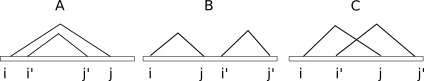
\includegraphics[scale=0.8]{possiblestr}
  \caption{A: $i < i' < j' < j$ B: $i < j < i' < j'$ C: $i < i' < j < j'$}
  \label{possiblestr}
\end{figure}

En la Figura~\ref{possiblestr} se pueden ver las posibles situaciones que se
pueden dar para dos pares $(i,j),(i',j')$ con $i < i'$. Seg\'un la definici\'on
que dimos m\'as arriba, las situaciones en $A$ y $B$ est\'an permitidas mientras
que la situaci\'on en $C$ representa un \textit{pseudo-knot} y estos no son
tenidos en cuenta.

\subsubsection{La estructura secundaria, el \ac{IRES} y la atenuaci\'on de un
virus}

La importancia de la estructura secundaria en este trabajo radica,
fundamentalmente, en su participaci\'on en la s\'intesis de prote\'inas del
virus y en consecuencia, en su atenuaci\'on. Para diferentes virus \ac{RNA}, se
puede decir que la estructura secundaria del \ac{IRES}, determina la
``afinidad'' o ``atracci\'on'' con los ribosomas. Luego, esto incide fuertemente
en el proceso de traducci\'on de las prote\'inas que causan la enfermedad, o que
est\'an involucradas en el proceso de replicaci\'on del virus. Una estructura
secundaria con menor afinidad (que la estructura secundaria del virus), le
permitir\'ia al sistema inmune generar los anticuerpos necesarios para
protegerse del virus antes de que se produzca la enfermedad.

\section{Los virus \ac{RNA}}
\label{virus}
Un virus \ac{RNA} es, esencialmente, aquel que tiene el \ac{RNA} como su
material gen\'etico. Adem\'as, los virus suelen clasificarse seg\'un la
``Clasificaci\'on de Baltimore'' que los agrupa en diferentes clases (clase I a
clase VII) seg\'un el tipo de genoma. En particular, en este trabajo se
contemplan los virus \ac{RNA} clase IV tambi\'en llamados \ac{(+)ssRNA virus}

Como ya se mencion\'o en la secci\'on~\ref{motivacion}, una de las
caracter\'isticas de este tipo de virus es su alta frecuencia de mutaciones.
Esto se debe, principalmente, a la alta tasa de error en su \ac{RNA}
polimerasa\footnote{A diferencia de la \ac{DNA} polimerasa que posee la
capacidad de detectar y corregir errores.} (involucrada en el proceso de
replicaci\'on del virus), estimada entre $1\times10^{-3}$ a $1\times10^{-5}$
errores por nucle\'otido por ciclo de replicaci\'on\cite{Vignuzzi08}. Debido a
que los virus de \ac{RNA} suelen tener menos de 10,000 nucle\'otidos, esto se
traduce en 0.1 a 10 mutaciones por genoma replicado.

Si retomamos lo dicho en la secci\'on~\ref{estructura} sobre la ``afinidad''
entre la estructura secundaria y los ribosomas, y c\'omo esto impacta en la
atenuaci\'on del virus, se puede ver que esta alta frecuencia de mutaciones,
conduce a la posibilidad de que en sucesivas replicaciones, el virus sufra
mutaciones que le devuelvan su estructura secundaria original (o similar) y en
consecuencia, pierda su atenuaci\'on.

\subsubsection{Poliovirus}

El poliovirus es un \ac{(+)ssRNA virus} de aproximadamente 7,500 nucle\'otidos
de longitud, miembro del g\'enero \textit{Enterovirus} de la familia
\textit{Picornaviridae} y causante de la poliomielitis. El poliovirus puede
atacar el sistema nervioso y destruir las c\'elulas nerviosas encargadas del
control de los m\'usculos. Como consecuencia, los m\'usculos afectados dejan de
cumplir su funci\'on y se puede llegar a una par\'alisis irreversible. En casos
severos, la enfermedad puede conducir a la muerte.

\subsubsection{La vacuna \ac{OPV}}

Ya presentamos en la secci\'on~\ref{motivacion} a la vacuna \ac{OPV} contra la
poliomielitis y sus principales complicaciones. Con los conceptos vistos
hasta el momento, estamos en condiciones de profundizar sobre el
porque de estas complicaciones.

Se han identificado tres serotipos\footnote{A los fines pr\'acticos y relevantes
en este trabajo, formas en que se presenta un determinado virus.} de poliovirus:
\ac{PV1}, \ac{PV2} y \ac{PV3}. Los tres serotipos son extremadamente virulentos
y producen los mismos s\'intomas de la enfermedad. Para cada uno de estos
serotipos, se desarroll\'o  su correspondiente virus atenuado Sabin 1, Sabin 2 y
Sabin 3 respectivamente que luego fueron combinados en la vacuna \ac{OPV}.

Cada uno de estos virus atenuados presentan diferentes niveles de riesgo o
probabilidad de revertir a la virulencia. El 90\% de los casos registrados de
\ac{VAPP} son causados por Sabin 2 o Sabin 3, mientras que tan solo el 10\%
restante, es causado por Sabin 1\cite{Philip92}. Esto se atribuye,
principalmente, a la cantidad de bases de nucle\'otidos en que difieren cada
serotipo con respecto a su correspondiente virus atenuado. Mientras que la
atenuaci\'on en Sabin 2 y Sabin 3 est\'a dada por el impacto de dos
o a lo sumo tres mutaciones, la atenuaci\'on en Sabin 1 es mas compleja y esto
justificar\'ia su menor probabilidad de revertir a la virulencia\cite{Philip92}.

M\'as all\'a de estas diferencias, los tres virus atenuados, Sabin 1, Sabin 2 y
Sabin 3, presentan mutaciones en la 5'-\ac{UTR} que contribuyen a la
atenuaci\'on. Adem\'as, de los aproximadamente 740 nucle\'otidos de la
5'-\ac{UTR}, los primeros 620 se conservan en todos los poliovirus, mientras que
las 100 bases que preceden el \ac{ORF} son las m\'as divergentes. Todo esto
sugiere que la 5'-\ac{UTR} tiene un rol muy importante en el ciclo de vida de
los poliovirus\cite{Philip92}.


\chapter{Bioinform\'atica y Biolog\'ia computacional}
\label{bioinformatica}
\epigraph{I can't be as confident about computer science as I can about biology.
Biology easily has 500 years of exciting problems to work on. It's at that
level.}%
{Donald Knuth}

Por tratarse de una disciplina relativamente nueva, nos permitimos una breve
introducci\'on, definici\'on y repaso de los principales problemas abordados
por la misma profundizando en aquellos problemas que est\'an directamente
relacionados con este trabajo. En particular, la predicci\'on de estructura
secundaria.

\section{Bio*}

La biolog\'ia depende en gran parte de la qu\'imica para poder avanzar y esto
dio lugar a lo que se conoce como \textit{bioqu\'imica}. An\'alogamente, la
necesidad de explicar fen\'omenos biol\'ogicos a nivel at\'omico, dio lugar a la
\textit{biof\'isica}. La \textit{biomatem\'atica} por su parte, se enfoca en el
modelado de procesos biol\'ogicos utilizando t\'ecnicas matem\'aticas que
permitan simular y predecir su comportamiento. La enorme cantidad de datos
recopilados por los bi\'ologos y la necesidad de herramientas para
interpretarlos, dio origen a lo que hoy conocemos como
\textit{bioinform\'atica}.

La bioinform\'atica fue precedida por lo que se llam\'o, \textit{biolog\'ia
computacional}. Aunque no hay una definici\'on precisa para ninguno de
los dos t\'erminos, la biolog\'ia computacional se caracterizo por enfocarse
en los aspectos te\'oricos/formales de las Ciencias de la Computaci\'on,
mientras que la bioinform\'atica supo estar mas relacionada con el
procesamiento de grandes vol\'umenes de datos, usualmente, almacenados en la
Internet. Actualmente, se suele hacer referencia a ambos t\'erminos de manera
indiferente.

\subsubsection{Problemas cl\'asicos}

A continuaci\'on presentamos algunos de los problemas o temas de investigaci\'on
abordados por la bioinform\'atica.

\begin{itemize}
 \item \textbf{An\'alisis de secuencias de \ac{DNA} o \ac{RNA}}. TBD
 \item \textbf{Dise\~no de secuencias de \ac{DNA} o \ac{RNA}}. TBD
 \item \textbf{Predicci\'on de interacci\'on entre prote\'inas}. TBD
\end{itemize}

\section{Predicci\'on de estructura secundaria}

Uno de los problemas que omitimos mencionar anteriormente y que describiremos
con mayor detalle, es el que se conoce como ``predicci\'on de estructura
secundaria''. 

Este problema consiste en, dada una estructura primaria o secuencia de \ac{RNA},
determinar la estructura secundaria correspondiente. Adem\'as, diferentes
secuencias de \ac{RNA} pueden tener la misma estructura secundaria, por lo que
tambi\'en nos interesa determinar para una estructura secundaria dada, las
secuencias de \ac{RNA} que conservan esa estructura. 

En ingles, se suele denominar a estos dos problemas ``folding'' e
``inverse folding'' respectivamente. A continuaci\'on describimos brevemente las
diferentes aproximaciones a cada uno de ellos.

Por lo mencionado en la secciones~\ref{estructura} y \ref{virus}, predecir la
estructura secundaria de una secuencia de \ac{RNA} y conocer las posibles
secuencias que conservan una estructura secundaria determinada, es de gran
importancia en este trabajo.

\subsection{Predicci\'on directa (folding)}
\label{folding}
Existen esencialmente 2 tipos de algoritmos para determinar o predecir la
estructura secundaria de una secuencia de \ac{RNA}.

\begin{itemize} 
 \item \textbf{Predicci\'on por \ac{mfe}}. Propuesto e implementado por Michael
Zuker en 1981\cite{Zuker81}, utiliza programaci\'on din\'amica para encontrar la
estructura secundaria que minimiza la energ\'ia libre.
 \item \textbf{Predicci\'on comparativa}. Utiliza diferentes m\'etodos para
comparar secuencias y estructuras con el fin de obtener una estructura por
``consenso''\cite{Gardner04}.
\end{itemize}

Si bien la ``predicci\'on comparativa'' presenta un incremento en la fidelidad
de los resultados obtenidos con respecto a la ``predicci\'on por \ac{mfe}''
\cite{Gardner04}, este tipo de algoritmos requieren la existencia de un conjunto
de secuencias relacionadas entre si (homologas) y esto no siempre es posible. En
particular para este trabajo nos interesa poder realizar predicciones de la
estructura secundaria a partir de una sola secuencia, por lo que la
``predicci\'on comparativa'' fue descartada.

Entre las implementaciones de la ``predicci\'on por \ac{mfe}'', se destacan
\textbf{RNAfold}\cite{Hofacker94} y \textbf{Mfold}\cite{Zuker81}. Ambas
implementan el algoritmo propuesto por Michael Zuker con complejidad
$\mathcal{O}(N^{3})$ donde $N$ es la longitud de la secuencia, aunque
\textbf{RNAfold} se presenta como una versi\'on mejorada y mas eficiente en la
pr\'actica. Como ya mencionamos en la secci\'on~\ref{estructura}, para lograr
esta complejidad polinomial, es necesario suponer la ausencia de
\textit{pseudo-knots}. De lo contrario, esta demostrado que el problema es
NP-completo\cite{Lyngso00}.

A continuaci\'on, se puede ver un ejemplo de una predicci\'on realizada con
\textbf{RNAfold}.

\begin{verbatim}
sancho@mulata:~$ RNAfold

Input string (upper or lower case); @ to quit
....,....1....,....2....,....3....,....4....,....5....,....6....,....7....,....8
AAAGGCAACGGCCAU
length = 15
AAAGGCAACGGCCAU
...(((....)))..
 minimum free energy =  -4.40 kcal/mol
\end{verbatim}

El resultado obtenido es precisamente, la energ\'ia libre y la estructura
secundaria representada con par\'entesis y puntos. Donde los pares de
par\'entesis indican las bases ``apareadas'' o ``unidas'' y los puntos, las
bases libres.

\subsection{Predicci\'on inversa (inverse folding)}
\label{inverse}
Las principales implementaciones que abordan este problema, lo plantean como un
\ac{CSP} y utilizan variantes de b\'usqueda local estoc\'astica para
resolverlo. La funci\'on objetivo y que se desea minimizar, es la distancia
estructural\footnote{Existen diferentes m\'etodos y algoritmos para calcular
la distancia entre estructuras cuya descripci\'on exceden este trabajo.}
entre la estructura \ac{mfe} de la secuencia soluci\'on\footnote{En este
contexto, una secuencia soluci\'on es aquella cuya predicci\'on de estructura
secundaria da como resultado la estructura buscada.} y la estructura secundaria
dada. 

Si bien la complejidad de este problema no esta determinada, a diferencia de
otros \ac{CSP}, la evaluaci\'on de las posibles soluciones es muy costosa ya que
implica la ``predicci\'on \ac{mfe}'' sobre cada secuencia candidata
($\mathcal{O}(N^{3})$). Luego, se deben utilizar diferentes t\'ecnicas que
tiendan a minimizar el numero de predicciones realizadas sobre la secuencia
completa.

En general, las diferentes implementaciones tienen como par\'ametros de
entrada, la estructura secundaria y opcionalmente, una secuencia de \ac{RNA}
incompleta (algunas bases indefinidas, generalmente representadas con la
letra N). Se distinguen dos pasos o etapas principales, que marcan las
diferencias entre una y otra implementaci\'on:
\begin{enumerate}
 \item \textbf{Inicializaci\'on:} determinar una secuencia inicial completando
la secuencia dada como par\'ametro. En el caso de no recibir ninguna secuencia
como par\'ametro, se asume una secuencias con todas las bases indefinidas.
 \item \textbf{B\'usqueda local:} mejorar iterativamente la secuencia inicial
hasta alcanzar una secuencia soluci\'on. Es decir, realizar cambios en la
secuencia que tiendan a minimizar la distancia estructural con la estructura
buscada.
\end{enumerate}

Entre estas implementaciones, se destacan \textbf{RNAinverse}\cite{Hofacker94},
\textbf{INFO-RNA}\cite{Busch07} y \textbf{RNA-SSD}\cite{Andronescu03}. Las
\'ultimas dos, se presentan como mejoras a la primera proponiendo diferentes
formas de generar la secuencia inicial e implementando algoritmos de b\'usqueda
local estoc\'astica mas complejos.

Notar que las tres implementaciones dependen de la generaci\'on de n\'umeros
\textit{pseudo aleatorios} y ya que la ``semilla'' utilizada es variable (salvo
\textbf{RNA-SSD} que permite fijar la semilla), se debe tener en cuenta el no
determinismo.

A continuaci\'on, mostramos un ejemplo de una predicci\'on inversa usando
\textbf{RNAinverse} sobre la estructura obtenida anteriormente con
\textbf{RNAfold}.

\begin{verbatim}
sancho@mulata:~$ RNAinverse 

Input structure & start string (lower case letters for const positions)
    @ to quit, and 0 for random start string
....,....1....,....2....,....3....,....4....,....5....,....6....,....7....,....8
...(((....)))..
aaaNNNNNNNNNNNu
length = 15
aaaUAGUCAGCUACu    3 0
\end{verbatim}

N\'otese que la secuencia obtenida, conserva las bases que ya estaban definidas
en la secuencia incompleta que se dio como par\'ametro y que adem\'as, es
distinta a la secuencia sobre la que se hizo la predicci\'on directa
anteriormente.

\chapter{Dise\~no de vacunas atenuadas}
\label{diseno}
\epigraph{Science is always wrong. It never solves a problem without creating
ten more.}%
{George Bernard Shaw}

Una vacuna atenuada es aquella que es creada reduciendo la virulencia de un
pat\'ogeno pero aun as\'i, manteni\'endolo viable (``vivo''). Antes de
adentrarnos en los detalles de lo que plantea este trabajo como metodolog\'ia
para racionalizar el dise\~no de vacunas atenuadas, veremos brevemente algunos
antecedentes y cu\'al fue, y sigue siendo, la metodolog\'ia cl\'asica para la
producci\'on de este tipo de vacunas.

\section{Dise\~no cl\'asico}

La metodolog\'ia para la producci\'on de vacunas atenuadas ha sido
hist\'oricamente el pasaje del virus a trav\'es de cultivos de c\'elulas
distintas a las c\'elulas hu\'esped. De esta manera, el virus tiende a
``evolucionar'' para adaptarse al nuevo hu\'esped y ser capaz de reproducirse.

Este concepto de ``evoluci\'on'', se traduce en alguna cantidad de mutaciones
sobre la secuencia de nucle\'otidos del virus y que se espera, reduzcan su
capacidad de reproducirse en el hu\'esped original. Luego, son precisamente
estas mutaciones las que le confieren la atenuaci\'on y dan lugar a la vacuna
atenuada.

La principal desventaja en este proceso es que las mutaciones que se producen
son totalmente impredecibles y a\'un cuando estas mutaciones derivan en un
virus atenuado, \'este podr\'ia revertir muy f\'acilmente a la virulencia
dependiendo de la naturaleza de las mutaciones que generan la
atenuaci\'on\cite{Badgett02}.
Adem\'as, como vimos en la secci\'on~\ref{virus}, la alta frecuencia de
mutaciones que poseen los virus \ac{RNA} aumenta la probabilidad de reversi\'on
a la virulencia. De hecho, esto es lo que ocurre con muchas vacunas atenuadas y
en particular, con la \ac{OPV}.

A pesar de este peligro de reversi\'on a la virulencia, \'esta sigue siendo la
principal metodolog\'ia para la producci\'on de vacunas atenuadas. Esto se debe,
fundamentalmente, a la falta de conocimiento sobre el significado o incidencia
de las mutaciones en la atenuaci\'on de un determinado virus. Sin embargo, los
recientes avances en la virolog\'ia molecular, han permitido explorar nuevas
t\'ecnicas que permitan controlar la replicaci\'on de un virus o su virulencia y
esto abri\'o la puerta a lo que se denomina ``dise\~no racional de vacunas
atenuadas''\cite{Lauring10}.

\section{Dise\~no racional}

La idea central en esta nueva metodolog\'ia, en la que se enmarca este trabajo,
es explotar el conocimiento que se ha producido en los \'ultimos a\~nos acerca
de la biolog\'ia molecular de determinados virus. Pudiendo controlar la
replicaci\'on de un virus o su virulencia, ser\'ia posible dise\~nar vacunas
atenuadas ``seguras'' evitando la impredecibilidad de las atenuaciones
emp\'iricas obtenidas mediante el dise\~no cl\'asico.

\subsection{Antecedentes}

Existen diferentes aproximaciones al dise\~no racional de vacunas
atenuadas\cite{Lauring10}. En general, todas estas aproximaciones se encuentran
en fase experimental y todav\'ia no se han aplicado en producci\'on. A
continuaci\'on hacemos menci\'on a tan solo dos de ellas, fundamentalmente para
marcar la diferencia con el dise\~no cl\'asico que presentamos anteriormente.

\subsubsection{Fidelidad en la replicaci\'on\cite{Vignuzzi08}} 

Como ya vimos en la secci\'on~\ref{virus}, la alta frecuencia de mutaciones en
los virus \ac{RNA} se debe a la alta tasa de error en su \ac{RNA} polimerasa.
Luego, modificando la \ac{RNA} polimerasa de tal manera que se reduzca su tasa
de error, se obtendr\'ia un virus atenuado mas estable y con menor probabilidad
de revertir a la virulencia en las sucesivas replicaciones. 

La principal desventaja de esta aproximaci\'on radica en que las
posibles variantes sobre la \ac{RNA} polimerasa deben ser determinadas y
evaluadas experimentalmente para cada virus en particular.

\subsubsection{(De-)Optimizaci\'on de codones\cite{Mueller10, Coleman08}} 

Si recordamos lo dicho en la secci\'on~\ref{bio-esencial} sobre el c\'odigo
gen\'etico, vimos que cada amino\'acido puede ser codificado hasta por 6
codones distintos. Es decir, distintas secuencias de nucle\'otidos resultan
equivalentes en t\'erminos de los amino\'acidos que codifican. Concretamente,
una prote\'ina de 300 amino\'acidos puede ser codificada por aproximadamente, 
$10^{151}$ secuencias de nucle\'otidos. 

Sin embargo, experimentalmente se pudo comprobar que algunos codones son m\'as
frecuentes que otros (\textit{codon bias}). Similarmente, pero de manera
independiente, se comprob\'o que determinados pares de codones son m\'as
frecuentes que otros (\textit{codon pair bias}). Aunque todav\'ia no est\'a
claro a qu\'e se debe esta ``parcialidad'' en el uso de codones o pares de
codones, se supone que afectar\'ia el proceso de s\'intesis de prote\'inas
(traducci\'on). 

Lo que se propone con esta aproximaci\'on, es determinar las secuencias de
nucle\'otidos que conserven la secuencia aminoac\'idica del virus pero que al
mismo tiempo, tiendan a usar codones y pares de codones menos frecuentes. De
esta manera, la atenuaci\'on del virus se obtendr\'ia debilitando su capacidad
de traducci\'on y replicaci\'on. 

Entre las ventajas que presenta esta metodolog\'ia, se destaca por un lado que
la atenuaci\'on es el resultado de un an\'alisis sistem\'atico y por lo tanto,
aplicable a diferentes virus de manera autom\'atica. Por otro lado, la alta
cantidad de cambios que se realizan sobre el virus original sugieren una menor
probabilidad de revertir a la virulencia.

\section{Propuesta de soluci\'on}
\label{vacunas-propuesta}

En pocas palabras, la propuesta consiste en encontrar un conjunto de secuencias
de \ac{RNA} que conserven las propiedades que le otorgan la atenuaci\'on al
virus y que, al mismo tiempo, tiendan a maximizar el n\'umero de mutaciones
necesarias para alcanzar secuencias semejantes a las pat\'ogenas o revertantes.

Esto tiene algunos puntos en com\'un con la ``(de-)optimizaci\'on de codones''
que presentamos anteriormente. En particular, ambas aproximaciones comparten la
idea de sistematizar el dise\~no de forma tal que pueda ser usado para
diferentes virus. Esto implica fundamentalmente, plasmar la metodolog\'ia en la
implementaci\'on de un software que, a partir de una serie de datos provistos
por el usuario, devuelva como resultado una o varias secuencias de nucle\'otidos
que representen posibles atenuaciones del virus.

De una forma m\'as abstracta, podemos pensar en un software para el dise\~no de
secuencias de nucle\'otidos basado en restricciones. Fundamentalmente, lo que se
busca es ``generar'' secuencias que satisfagan determinadas propiedades o
restricciones. En particular, aquellas que tiendan a reducir la virulencia del
virus.

En este sentido, se podr\'ia trazar una analog\'ia con los algoritmos para la
predicci\'on inversa de estructura secundaria (\textit{inverse folding}). En
esencia, estos algoritmos ``dise\~nan'' secuencias de \ac{RNA} que tengan como
estructura secundaria \ac{mfe}, la estructura dada por el usuario. De hecho,
como mencionamos en la secci\'on~\ref{inverse}, el problema se plantea
computacionalmente como un \ac{CSP}.

La principal innovaci\'on de esta propuesta es que las restricciones se enfocan
esencialmente en el \ac{IRES} y su estructura secundaria. Por lo visto en la
secci\'on~\ref{virus}, parece clara la importancia del \ac{IRES} en la
traducci\'on y posterior replicaci\'on de diferentes virus \ac{RNA} y en
particular del poliovirus.

Lo que nos proponemos en este trabajo, es realizar un an\'alisis sistem\'atico
de las posibles variantes al \ac{IRES} de los virus atenuados  Sabin (y
eventualmente cualquier otro) que conserven la estructura secundaria y
en consecuencia, la atenuaci\'on del virus. Luego, maximizando la cantidad de
mutaciones necesarias para revertir a secuencias semejantes a las pat\'ogenas o
revertantes, estar\'iamos reduciendo la probabilidad de que el virus atenuado
sufra reversi\'on a la virulencia.

Esquem\'aticamente, podr\'iamos plantear el problema de la siguiente manera:
\begin{itemize}
 \item \textbf{Entrada:} Genoma del virus atenuado, genomas de los pat\'ogenos
o revertantes y un conjunto de restricciones. Fundamentalmente, la
conservaci\'on de la estructura secundaria del \ac{IRES} del virus atenuado.
 \item \textbf{Objetivo:} Satisfaciendo las restricciones impuestas, maximizar
la distancia entre el genoma del virus atenuado y los genomas pat\'ogenos o
revertantes.
 \item \textbf{Salida:} Una o varias secuencias, candidatas a ``mejorar'' el
virus atenuado.
\end{itemize}

\subsection{Formalizaci\'on}
\label{formalizacion-prop}
Como mencionamos en la secci\'on~\ref{propuesta} esto puede ser visto como un
problema de \textbf{``optimizaci\'on combinatoria basado en restricciones''}.
Pero para hacerlo, primero se deben identificar algunos elementos fundamentales
que permitan definir el problema.

Repasando lo dicho en la secci\'on~\ref{propuesta}, este tipo de problemas
consiste en asignar valores a un conjunto finito de variables (componentes de
una soluci\'on) que satisfagan determinadas restricciones. En nuestro caso,
estas restricciones ser\'an propiedades biol\'ogicas sobre partes de una
secuencia de \ac{RNA}, y los posibles valores a asignar ser\'an (sub)secuencias
de \ac{RNA} que satisfagan las propiedades requeridas.

Sobre diferentes partes de la secuencia de \ac{RNA} se podr\'ian requerir
diferentes propiedades biol\'ogicas (restricciones). Luego, ser\'an estas
propiedades las que determinen los posibles valores sobre cada parte
``variable'' de la secuencia. Finalmente, las combinaciones de los posibles
valores para cada parte de la secuencia, formar\'an las potenciales soluciones
del problema.

\subsubsection{Definici\'on del problema}

Sea $N$ la longitud de la secuencia de \ac{RNA} del virus atenuado, y para $k
\in \mathbb{N}$ sea $\mathcal{S}_{k}$ el conjunto de secuencias de \ac{RNA} de
longitud $k$. Entonces definimos:

\begin{itemize} 
 \item \textbf{Espacio de soluciones:} $\mathcal{S}_{N}$

 \item \textbf{Componentes variables de una soluci\'on:} $s_{1},s_{2}, \dots,
s_{n}$ tal que $s_{i} \in \mathcal{S}_{N_{i}}$ con $1 \le i \le n$ y $0 < N_{i}
\le N$.

 \item \textbf{Restricciones sobre las componentes:} Conservaci\'on de la
estructura secundaria o de la secuencia aminoac\'idica con respecto al virus
atenuado. Eventualmente, se podr\'ian contemplar otras restricciones que
impliquen propiedades biol\'ogicas que resulten de inter\'es para la
atenuaci\'on del virus.

 \item \textbf{Funci\'on ``objetivo'' o de evaluaci\'on:} $f: \mathcal{S}_{N}
\rightarrow \mathbb{R}$ tal que $f(s)$ calcula la bondad de cada soluci\'on, en
nuestro caso, como la distancia en n\'umero de mutaciones necesarias para
llegar de $s$ a alguna secuencia pat\'ogena o revertante.
\end{itemize}

Lo primero que podemos mencionar es que para cualquier virus \ac{RNA}, recorrer
el espacio de soluciones de manera exhaustiva es inviable ya que por ejemplo,
para el caso del poliovirus, $N \simeq 7,500$. Es decir que existen
aproximadamente $4^{7,500}$ posibles secuencias de \ac{RNA} (7,500
posiciones y 4 bases de nucle\'otidos posibles para cada posici\'on).

Por otro lado, la posibilidad de evaluar los posibles valores para cada
componente $s_{i}$ de manera exhaustiva, depender\'a fundamentalmente del tipo
de restricci\'on impuesta sobre esa componente y de la longitud $N_{i}$. En
particular para los virus atenuados Sabin y la conservaci\'on de la estructura
secundaria del \ac{IRES} ($N_{i} \simeq 400$), la evaluaci\'on exhaustiva
ser\'ia inviable debido al alto costo de predecir la estructura secundaria,
como vimos en las secciones~\ref{folding} y \ref{inverse}.

Con el problema planteado de esta manera y debido a la inviabilidad de realizar
una b\'usqueda exhaustiva, se pueden utilizar diferentes algoritmos de
b\'usqueda local para que, partiendo de una secuencia de \ac{RNA} inicial, en
este caso el virus atenuado, recorrer el espacio de b\'usqueda $\mathcal{S}_{N}$
teniendo como objetivo, maximizar la funci\'on de evaluaci\'on $f$.

En este contexto, la definici\'on de la funci\'on de evaluaci\'on $f:
\mathcal{S}_{N} \rightarrow \mathbb{R}$ ser\'a crucial para encontrar buenas
soluciones. En principio se podr\'ia pensar que la imagen de la funci\'on, sea
$\mathbb{N}$ en lugar de $\mathbb{R}$. De hecho, este es el caso si la funci\'on
calcula la distancia de \textit{Hamming} est\'andar. Esto es, sumar 1 por cada
una de las bases en las que difiere la secuencia soluci\'on de la secuencia
pat\'ogena. Pero de esta manera se estar\'ia suponiendo que la probabilidad de
mutaci\'on entre las bases es uniforme y esto no es as\'i necesariamente. 

Luego, determinando emp\'iricamente la probabilidad de mutaci\'on de cada base
hacia cualquiera de las otras tres, se podr\'ia incluir esta informaci\'on en la
funci\'on de evaluaci\'on usando una matriz de dimensi\'on $4\times4$ indicando
en cada posici\'on $(i,j)$, el costo de realizar la mutaci\'on de la base $i$ a
la base $j$.

En particular, para la distancia de \textit{Hamming} podemos definir la
siguiente matriz de costos:
\[
M = 
\begin{Bmatrix}
 0 & 1 & 1 & 1\\
 1 & 0 & 1 & 1\\
 1 & 1 & 0 & 1\\
 1 & 1 & 1 & 0
\end{Bmatrix}
\]



\part{Desarrollo del Software}
\label{software}
\chapter{Proceso de desarrollo}
\epigraph{How does a project get to be a year late?... One day at a time.}%
{Fred Brooks}

A esta altura ya hemos presentado los principales conceptos biol\'ogicos
involucrados en este trabajo, el dise\~no de vacunas atenuadas y la
formalizaci\'on del problema que nos propusimos resolver. En los cap\'itulos
restantes veremos los aspectos t\'ecnicos mas relevantes sobre el desarrollo del
software.

\section{Modelo de desarrollo}

Para llevar adelante el desarrollo del software, se opto por el cl\'asico
modelo de cascada. Fundamentalmente debido a su simplicidad y a que los
requerimientos con que deb\'ia cumplir el software estaban bien definidos desde
el inicio. No solo a nivel funcional, sino tambi\'en en cuanto a principios del
dise\~no orientado a objetos.

\subsection{Etapas de la cascada}

Las etapas que se llevaron a cabo durante el desarrollo de este trabajo y que
veremos con mayor detenimiento en los siguientes cap\'itulos, fueron las
siguientes:
\begin{enumerate}
 \item Especificaci\'on de requerimientos.
 \item Dise\~no.
 \item Implementaci\'on.
 \item Verificaci\'on.
\end{enumerate}

Quedaron fuera del alcance, las etapas ``Instalaci\'on'' y por supuesto,
``Mantenimiento''.

\subsection{Consideraciones del modelo}

Para implementar el modelo de cascada se tuvieron en cuenta algunas
consideraciones con respecto al contexto en el que se desarroll\'o el software
y que veremos a continuaci\'on. 

Por un lado, todas las etapas que enumeramos m\'as arriba deb\'ian ser llevadas
a cabo por la misma persona. Esto es significativamente distinto a contar con
grupos de personas o equipos independientes para cada etapa y en donde la
documentaci\'on generada en cada fase es fundamental para la comunicaci\'on
entre los distintos equipos. En este sentido, usamos un modelo de cascada con
``solapamiento'', tambi\'en conocido como \textit{Sashimi}\cite{Mcconnell96},
que permite empezar una etapa sin haber terminado por completo la anterior.
Debido a que en este modelo es m\'as natural la continuidad del personal entre
las distintas etapas, no es necesario generar tanta documentaci\'on como en el
modelo de cascada ``puro'' y esto agiliz\'o el proceso de desarrollo.

Por otro lado, el rol de ``cliente'' en el proceso de desarrollo fue cubierto
por miembros de \ac{FuDePAN} que garantizaron el conocimiento del dominio de
manera tal de poder realizar la ``Especificaci\'on de requerimientos'' pero al
mismo tiempo, contaban con los conocimientos t\'ecnicos de dise\~no y
programaci\'on orientada a objetos como para supervisar el desarrollo en estos
aspectos. En este sentido, se tomaron algunos elementos de la variante al modelo
de cascada ``puro'' que se conoce como \textit{Staged
Delivery}\cite{Mcconnell96} o ``implementaci\'on incremental'' que nos
permitieron realizar revisiones peri\'odicas con miembros de \ac{FuDePAN}
durante las etapas de ``Dise\~no'' e ``Implementaci\'on''.

En la Figura~\ref{modelos} se pueden ver el modelo de cascada ``puro'' y las
variantes descriptas anteriormente y que adoptamos para este trabajo.

\begin{figure}
 \centering
  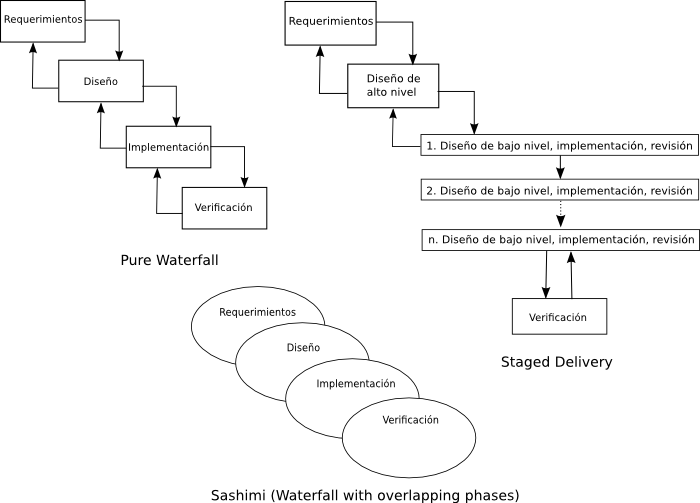
\includegraphics[scale=0.6]{modelos}
  \caption{Modelos de desarrollo}
  \label{modelos}
\end{figure}


Por \'ultimo, con el fin de validar los requerimientos del software que se
consideraban m\'as importantes, durante la etapa de ``Dise\~no'', se
implement\'o un prototipo utilizando el lenguaje de programaci\'on Python.

\section{Ecosistema}

El ``ecosistema'' de herramientas que se utilizaron para llevar adelante el
proceso de desarrollo son las siguientes:

\begin{itemize}
 \item \textbf{Lenguaje de programaci\'on:} El software se implemento en
\textbf{C++}\footnote{\url{http://cplusplus.com}}.
 \item \textbf{Lenguaje de dise\~no:} El dise\~no del software se hizo
utilizando \textbf{UML}\footnote{\url{http://www.uml.org}}.
 \item \textbf{Control de versiones:} Se utilizo el sistema de control de
versiones \ac{SVN}\footnote{\url{http://subversion.apache.org}} y puede ser
consultado en \url{http://vac-o.googlecode.com}.
 \item \textbf{Sistema de ``construcci\'on'':} Para automatizar el
proceso de compilaci\'on del c\'odigo fuente se
utilizo \textbf{CMake}\footnote{\url{http://www.cmake.org}}.
 \item \textbf{Automatizaci\'on de pruebas:} Para realizar la verificaci\'on del
software, se opto por implementar pruebas
unitarias utilizando
\textbf{google-test}\footnote{\url{http://googletest.googlecode.com}} y
\textbf{google-mock}\footnote{\url{http://googlemock.googlecode.com}}. 
 \item \textbf{An\'alisis est\'atico:} Se utilizaron las herramientas
\textbf{astyle}\footnote{\url{http://astyle.sourceforge.net}} y
\textbf{cppcheck}\footnote{
\url{http://sourceforge.net/apps/mediawiki/cppcheck}}.
 \item \textbf{An\'alisis din\'amico:} Se utilizaron las herramientas
\textbf{valgrind}\footnote{\url{http://valgrind.org}} y
\textbf{gcov}\footnote{\url{http://gcc.gnu.org/onlinedocs/gcc/Gcov.html}} para
verificar la ausencia de ``memory leaks'' y la cobertura de las pruebas.
\end{itemize}

\chapter{Requerimientos}
\epigraph{If you think it's simple, then you have misunderstood the problem.}%
{Bjarne Stroustrup}

Los requerimientos del software fueron provistos por miembros de \ac{FuDePAN} y
quedaron documentados en la ``Especificaci\'on de Requerimientos de Software''
que se anexa a este trabajo. A continuaci\'on haremos menci\'on a los
requerimientos mas relevantes y que nos permitan introducir los principales
aspectos del software.

\section{Descripci\'on general}

Retomando lo dicho en la secci\'on~\ref{vacunas-propuesta}, podr\'iamos
resumir los requerimientos funcionales de \ac{vac-o} de la siguiente manera:

\begin{itemize}
 \item \textbf{Entrada:} Genoma del virus atenuado, genoma del pat\'ogeno o
revertantes y un conjunto de restricciones sobre partes de la secuencias del
virus atenuado.
 \item \textbf{Objetivo:} Satisfaciendo las restricciones impuestas, maximizar
la cantidad de mutaciones necesarias para convertir el virus atenuado en alguna
secuencia pat\'ogena o revertante.
 \item \textbf{Salida:} Una o varias secuencias, candidatas a ``mejorar'' el
virus atenuado.
\end{itemize}

Desde el punto de vista del dise\~no, el sistema deb\'ia ser altamente modular,
de forma que sea apto para encontrar secuencias gen\'omicas para diferentes
tipos de organismos. En este sentido, se debieron seguir los principios de
dise\~no conocidos por el acr\'onimo \textbf{SOLID}\cite{Martin00}.

\section{Extensiones}

Uno de los principales requerimientos con que deb\'ia cumplir el software es
que sea vers\'atil. Es decir, que permita ser configurado y extendido de una
forma simple y sin modificar sus componentes centrales.

En este sentido, se propuso desde un comienzo un software que funcionar\'ia en
base a la informaci\'on provista por una extensi\'on o \textit{plugin}.
B\'asicamente, la responsabilidad de una extensi\'on ser\'ia la de proveer a
\ac{vac-o} la informaci\'on relevante para cada virus atenuado que se desee
optimizar. En particular, el genoma del virus atenuado, el genoma del
pat\'ogeno y el conjunto de restricciones que se deben satisfacer durante la
b\'usqueda. Las extensiones tambi\'en ser\'ian responsables de evaluar las
secuencias candidatas y de determinar la estrategia de b\'usqueda.


\section{Regiones combinatorias}

Como ya mencionamos anteriormente, el problema se puede ver como un problema de
``optimizaci\'on combinatoria basado en restricciones''. Luego, un ingrediente
que no podemos dejar de mencionar son precisamente, las restricciones o
``regiones combinatorias''. Fundamentalmente, representan las componentes
variables de cada soluci\'on y definen en gran medida el espacio de b\'usqueda.

En este contexto nos referimos a las ``variantes'' de una regi\'on como los
posibles valores (secuencias de \ac{RNA}) que satisfacen la restricci\'on
impuesta. Luego podemos definir a una regi\'on combinatoria de la siguiente
manera.
\begin{definition}
\label{region}
Dada una secuencia de \ac{RNA} $S$ de longitud $n$, una regi\'on combinatoria
sobre $S$ sera una 4-upla $(inicio, fin, tipo, eval)$ tal que:
\begin{itemize}
 \item $0 \le inicio < fin \le n$
 \item $tipo$ determina la restricci\'on sobre la regi\'on y por ende, queda
definido un conjunto $\mathcal{V}$ de posibles variantes a la regi\'on.
 \item $eval: \mathcal{V} \rightarrow (0,1)$ es una funci\'on de evaluaci\'on
local a la regi\'on que determina la bondad de una variante determinada.
\end{itemize}
\end{definition}

Si suponemos $N \ge 1$ y $R_{1}, \dots, R_{N}$ regiones combinatorias.
Entonces tendremos que el n\'umero de posibles secuencias que \ac{vac-o}
``deber\'ia'' evaluar, sera igual al producto cartesiano $\mathcal{V}_{1} \times
\dots \times \mathcal{V}_{N}$ con  $\mathcal{V}_{1}, \dots, \mathcal{V}_{N}$
variantes de cada regi\'on combinatoria respectivamente.

Inicialmente, se contemplaron dos tipos de regiones combinatorias aunque se debe
tener en cuenta la posibilidad de que en el futuro se agreguen mas. Estos tipos
de regiones combinatorias o restricciones son:
\begin{itemize}
 \item Conservaci\'on de la estructura secundaria de \ac{RNA}.
 \item Conservaci\'on del c\'odigo gen\'etico.
\end{itemize}

Adem\'as, para el caso de la ``conservaci\'on de estructura secundaria de
\ac{RNA}'' se deb\'ia contar con la posibilidad de utilizar diferentes
algoritmos de predicci\'on directa e inversa de manera ``transparente''.

\section{Estrategias de b\'usqueda}

Otro de los aspectos ``configurables'' del software deb\'ia ser la estrategia
de b\'usqueda utilizada. En este sentido, la extensi\'on es responsable de
proveer al sistema la ``forma'' de recorrer el espacio de b\'usqueda y al mismo
tiempo determinar cuando se debe terminar el recorrido.

Vale aclarar que todos los algoritmos de b\'usqueda local son ``incompletos''
en el sentido de que no recorren exhaustivamente el espacio de b\'usqueda como
si lo hacen los algoritmos mas tradicionales o sistem\'aticos. Luego, es
necesario contar con un criterio de terminaci\'on que suele estar relacionado
con la cantidad de iteraciones realizadas, la ``calidad'' de las soluciones
encontradas o la cantidad de iteraciones sin que se produzcan mejores
soluciones.

\section{Control de calidad}

Cada secuencia encontrada por \ac{vac-o} durante el recorrido del espacio
de b\'usqueda, debe ser sometida a un ``control de calidad''. B\'asicamente
se pretende simular las mutaciones acumuladas que se producen en las sucesivas
replicaciones del virus en la naturaleza y sobre cada secuencia mutante,
verificar determinadas propiedades que brinden mayor seguridad sobre la
atenuaci\'on del virus.

An\'alogamente a las regiones combinatorias, definimos las regiones de
validaci\'on de la siguiente manera.

\begin{definition}
Dada una secuencia de \ac{RNA} $S$ de longitud $n$, una regi\'on de validaci\'on
sobre $S$ sera una 4-upla $(inicio, fin, prueba, criterio)$ tal que:
\begin{itemize}
 \item $0 \le inicio < fin \le n$
 \item $prueba$ determina la forma en que se producen las mutaciones.
 \item $criterio$ determina la propiedad que deben cumplir todas las secuencias
mutantes generadas.
\end{itemize}
\end{definition}

Se puede pensar al control de calidad como la generaci\'on de un \'arbol de
secuencias. La ra\'iz del \'arbol sera la secuencia candidata y los nodos del
\'arbol ser\'an las secuencias mutantes generadas. Luego, diremos que una
secuencia candidata pasa el control de calidad sobre una regi\'on de
validaci\'on, cuando sea posible generar todos los nodos del \'arbol para una
profundidad dada. Por ultimo, solo ser\'an consideradas aquellas secuencias
candidatas que pasen el control de calidad sobre todas las regiones de
validaci\'on.

Para las formas de producir mutaciones acumuladas se contemplaron dos
alternativas:
\begin{itemize}
 \item Mutaciones sistem\'aticas.
 \item Mutaciones aleatorias.
\end{itemize}

Por otro lado, las propiedades que se contemplaron como criterio de
verificaci\'on son:
\begin{itemize}
 \item Similitud estructural.
 \item Disimilitud estructural.
\end{itemize}

De todas formas, se deb\'ia contemplar la posibilidad de que en el
futuro se agreguen otras formas de generar mutaciones y otros criterios de
verificaci\'on.

\section{Ranking de secuencias candidatas}

Finalmente, nos queda por describir el ranking de secuencias candidatas y que
representa fundamentalmente el resultado de la ejecuci\'on de \ac{vac-o}.

Esto es simplemente un listado de secuencias de \ac{RNA}, ordenadas seg\'un la
evaluaci\'on que hiciera la extensi\'on. B\'asicamente, las secuencias mejor
evaluadas ser\'an aquellas que est\'en a mayor distancia (para alguna
definici\'on de distancia) de la secuencia pat\'ogena o revertante y por ende,
tendr\'an menor probabilidad de sufrir reversi\'on a la virulencia.
\chapter{Dise\~no}
\epigraph{The effective exploitation of his powers of abstraction must be
regarded as one of the most vital activities of a competent programmer.}%
{Edsger W. Dijkstra}

Al igual que con los requerimientos del software, la descripci\'on detallada del
dise\~no quedo documentada en la ``Especificaci\'on de Dise\~no de Software'' y
que se agrega como anexo. An\'alogamente al capitulo anterior, nos limitaremos
a mencionar solo los aspectos mas relevantes del dise\~no, dejando como lectura
adicional el documento anexo.

\section{Metodolog\'ia}

La metodolog\'ia adoptada para realizar el an\'alisis y descripci\'on del
dise\~no se denomina \ac{RDD}\cite{Wirfs03}. Esta t\'ecnica del dise\~no
orientado a objetos, se enfoca en qu\'e responsabilidades deben ser
cubiertas por el sistema y en cu\'ales ser\'an los objetos responsables de
llevarlas a cabo.

Por ``responsabilidades'' se entiende fundamentalmente lo siguiente:
\begin{itemize}
 \item Las acciones que realiza un objeto.
 \item El conocimiento o la informaci\'on que mantiene un objeto.
 \item Las decisiones que realiza un objeto afectando a otros.
\end{itemize}

\subsubsection{Objetivos del dise\~no}

Como ya mencionamos anteriormente, uno de los requerimientos del software fue
que se respetaran los principios del dise\~no orientado a objetos resumidos en
el acr\'onimo \textbf{SOLID}\cite{Martin00}.
\begin{itemize}
  \item \ac{SRP}
  \item \ac{OCP}
  \item \ac{LSP}
  \item \ac{ISP}
  \item \ac{DIP}
\end{itemize}

En particular se puso especial atenci\'on en respetar los principios \ac{SRP}, 
\ac{OCP} y \ac{DIP} debido a que repercuten directamente en que el sistema sea
mas simple de mantener y extender con nuevas funcionalidades. Adem\'as, el
principio \ac{DIP} es fundamental para lograr un software que sea verificable
mediante la automatizaci\'on de pruebas como se pudo comprobar mas adelante, en
la etapa de ``verificaci\'on''.

\section{Arquitectura}

A continuaci\'on veremos los principales componentes del sistema y siguiendo la
metodolog\'ia adoptada, sus respectivas responsabilidades. En la
Figura~\ref{arquitectura} se puede ver el diagrama UML correspondiente. 

\begin{figure} 
  \centering
  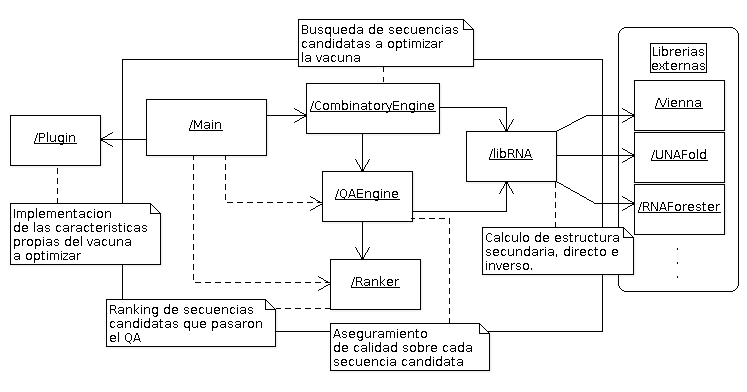
\includegraphics[scale=0.5]{architecture.png}
  \caption{Arquitectura de vac-o.}
\label{arquitectura}
\end{figure}

\begin{itemize}
   \item \textbf{Main:} Representa el componente principal en t\'erminos de
ejecuci\'on del sistema. Comprende principalmente, la inicializaci\'on y
configuraci\'on de otros componentes.
   \item \textbf{Plugin:} Representa la implementaci\'on de las
caracter\'isticas propias de la vacuna que se desea optimizar. Brinda
informaci\'on para la configuraci\'on inicial como as\'i tambi\'en, los
criterios para evaluar las secuencias candidatas.
   \item \textbf{CombinatoryEngine:} Representa el motor combinatorio del
sistema encargado de encontrar, nuevas secuencias que sean candidatas a
optimizar la atenuaci\'on del virus.
   \item \textbf{QAEngine:} Representa el motor de control de calidad del
sistema encargado de decidir, si una secuencia candidata pasa el control o no.
   \item \textbf{Ranker:} Representa el componente encargado de mantener un
``ranking'' de secuencias que sera adem\'as, el resultado final de la
ejecuci\'on.
   \item \textbf{libRNA:} Representa el componente que provee al sistema
funcionalidades para la manipulaci\'on de secuencias y estructuras de \ac{RNA}
(``folding'' directo e inverso y comparaci\'on estructural, entre otras)
utilizando librer\'ias externas.
  \end{itemize}

En las siguientes secciones profundizaremos sobre los componentes ``libRNA'' y
``CombinatoryEngine'' por ser probablemente los mas importantes en cuanto a sus
responsabilidades y dejaremos como lectura adicional la ``Especificaci\'on de
Dise\~no de Software'' que contiene una descripci\'on detallada de todos los
componentes de la arquitectura presentada. Al mismo tiempo, profundizar sobre
estos componentes, nos permitir\'a introducir los principales patrones de
dise\~no que se utilizaron de forma an\'aloga en otras partes del sistema.
Entre otros, se destacan \textit{Iterator}, \textit{Observer}, \textit{Template
Method} y \textit{Visitor}. Para una descripci\'on de estos y otros patrones
del dise\~no orientado a objetos, ver \cite{Gamma95}.

\section{Librer\'ias externas}
\label{diseno-libRNA}
Como vimos en la secciones~\ref{folding} y \ref{inverse}, existen diversas
implementaciones que resuelven el problema de la predicci\'on (directa e
inversa) de estructura secundaria de \ac{RNA} y lo mismo ocurre para el caso de
la comparaci\'on estructural. Adem\'as no se descarta la posibilidad de que en
el futuro aparezcan nuevas y mejores implementaciones. 

Por todo esto, uno de los requerimientos del software fue que sea posible el uso
de cualquiera de estas implementaciones de manera transparente. El problema
radica en que cada librer\'ia tiene diferentes formas de recibir los
par\'ametros de entrada y diferentes formas de dar los resultados que genera. A
ra\'iz de esto se propuso el componente ``libRNA'' como una forma de unificar el
acceso a estas librer\'ias externas e integrarlas al resto del sistema. Las
interfaces propuestas fueron las siguientes:

\begin{itemize}
 \item \textbf{IFold:} Provee la predicci\'on directa (\textit{folding})
de secuencias de \ac{RNA}.
 \item \textbf{IFoldInverse:} Provee la predicci\'on inversa (\textit{inverse
folding}) de secuencias de \ac{RNA}.
 \item \textbf{IStructureCmp:} Provee la comparaci\'on de estructuras
secundarias
de \ac{RNA}.
 \item \textbf{ISequenceCmp:} Provee la comparaci\'on de secuencias de
\ac{RNA}.
\end{itemize}

En esto podemos ver la idea del principio de dise\~no \ac{DIP}. Haciendo que el
sistema dependa de estas interfaces en lugar de sus respectivas
implementaciones conseguimos abstraer los detalles de cada librer\'ia externa y
logramos un software mas vers\'atil. En el capitulo~\ref{librerias} veremos
algunos detalles sobre las implementaciones de estas interfaces y en particular
de \textbf{IFoldInverse}.

\section{Motor combinatorio}

El componente ``CombinatoryEngine'' contiene todo lo referente al recorrido del
espacio de b\'usqueda por lo que es claramente, uno de los componentes
principales de \ac{vac-o}. Esto es fundamentalmente, las regiones
combinatorias y las diferentes estrategias de b\'usqueda.

Para permitir que el software sea de utilidad para diferentes tipos de virus,
tanto las regiones combinatorias como la estrategia de b\'usqueda utilizada
para la optimizaci\'on, deb\'ian ser altamente configurables. Luego, el
objetivo sobre este componente, fue capturar la estructura general de los
algoritmos de b\'usqueda local que suelen denominarse de ``mejoramiento
iterativo''. Algunos de estos algoritmos son:

\begin{itemize}
 \item \textit{First Improvement}
 \item \textit{Best Improvement}
 \item \textit{Simulated Annealing}
 \item \textit{Tabu Search}
\end{itemize}

En todos estos algoritmos, y en general en la b\'usqueda local, est\'an
presentes los conceptos de ``vecindario'' (\textit{neighborhood}) y de
``movimiento'' (\textit{step}) que veremos con mayor detenimiento en el
capitulo~\ref{busqueda}. Mientras tanto, la siguiente introducci\'on nos
servir\'a para justificar las interfaces propuestas.

Si el espacio de b\'usqueda es $\mathcal{S}$, entonces un ``vecindario'' sera
una relaci\'on $\mathcal{N} \subseteq \mathcal{S} \times \mathcal{S}$ y el
``movimiento'' (entre soluciones en el espacio de b\'usqueda) sera una funci\'on
$step: \mathcal{S} \rightarrow \mathcal{D}(\mathcal{S})$. Donde $\mathcal{D}(S)$
denota el conjunto de distribuciones de probabilidad sobre un conjunto dado $S$
y donde una distribuci\'on de probabilidad $D \in \mathcal{D}(S)$ es una
funci\'on $D:S \rightarrow \mathbb{R}^{+}_{0}$ que mapea los elementos de $S$ a
sus respectivas probabilidades.

Luego, en cada iteraci\'on de la b\'usqueda, hay dos responsabilidades bien
diferenciadas e independientes. Por un lado, se debe explorar el ``vecindario''
de la soluci\'on actual. Es decir, si la soluci\'on actual es $s$ y el
``vecindario'' es $\mathcal{N}$, debemos generar el conjunto de soluciones
$\mathcal{N}(s)$. Por otro lado, una vez que se tiene el conjunto
$\mathcal{N}(s)$ de ``vecinos'' de $s$, se debe seleccionar uno de ellos
utilizando la funci\'on $step$. Notar que no siempre la soluci\'on seleccionada
sera mejor que la soluci\'on actual. Inclusive los algoritmos que permiten los
llamados, ``movimientos malos'' (seleccionar con una probabilidad $p$ una
soluci\'on peor que la actual) suelen conducir a mejores resultados.

En este sentido se propusieron la siguientes interfaces:

\begin{itemize}
 \item \textbf{ICombinatoryRegion:} Genera las variantes de la regi\'on
combinatoria que satisfagan la restricci\'on asociada.
 \item \textbf{ISolution:} Representa una soluci\'on en el espacio de
b\'usqueda.
 \item \textbf{INeighborhood:} Explora el vecindario de una soluci\'on.
 \item \textbf{IStrategy:} Decide como pasar de una soluci\'on a la siguiente y
notifica las soluciones que ``mejoran'' a la soluci\'on anterior.
 \item \textbf{ICombinatoryEngine:} Inicia la b\'usqueda y notifica a otros
componentes del sistema las sucesivas soluciones encontradas.
\end{itemize}

Para terminar de entender la interacci\'on entre estas interfaces, en la
Figura~\ref{motor} se puede ver el diagrama de secuencia del motor combinatorio.

\begin{figure} 
  \centering
  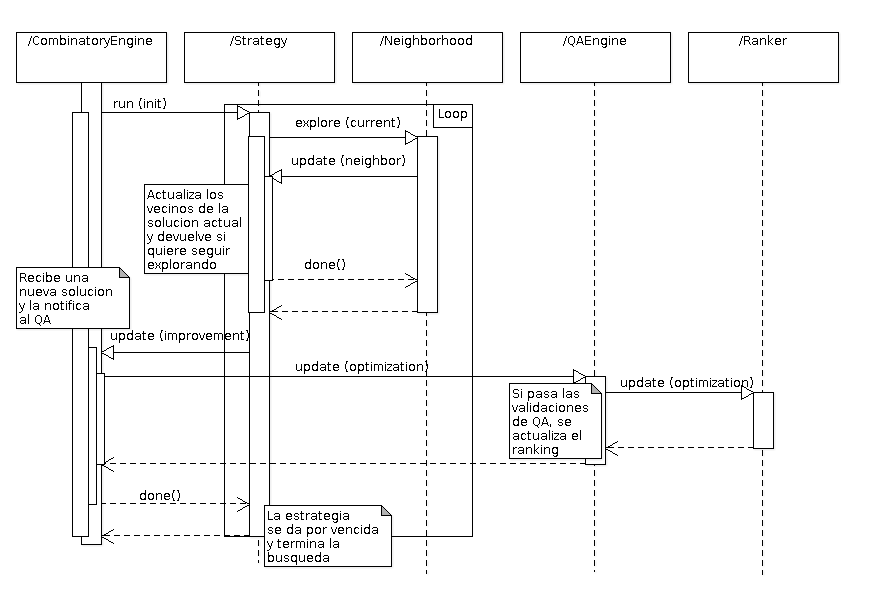
\includegraphics[scale=0.45]{sequence.png}
  \caption{Motor combinatorio de vac-o.}
\label{motor}
\end{figure}

El principal patr\'on de dise\~no que utilizamos en este componente es el que
se denomina \textit{Observer} y que sirve fundamentalmente para lograr la
comunicaci\'on entre diferentes objetos sin que se produzca acoplamiento. La
idea es establecer una relaci\'on entre un emisor y uno, o varios receptores
sin necesidad de generar una dependencia entre el objeto emisor y el objeto
receptor. Adem\'as para permitir el uso del patr\'on \textit{Observer} entre
diferentes tipos de objetos, se propuso el patr\'on de dise\~no \textit{Template
Method}.

En nuestro caso, \textbf{INeighborhood} notifica a \textbf{IStrategy} por cada
soluci\'on que se genera mientras se explora el vecindario de la soluci\'on
actual. Posteriormente, si la soluci\'on seleccionada es mejor que la soluci\'on
actual, \textbf{IStrategy} notifica a \textbf{ICombinatoryEngine} la soluci\'on
seleccionada y este a su vez, la notifica a otros componentes de \ac{vac-o}
(control de calidad).

Una vez mas, remarcamos que las dependencias son entre interfaces y no entre
implementaciones como establece el principio de dise\~no \ac{DIP}. Esto nos
brinda la versatilidad de definir diferentes tipos de regiones combinatorias y
estrategias de b\'usqueda sin modificar en absoluto la implementaci\'on del
motor combinatorio.
\chapter{Predicci\'on directa e inversa de estructura secundaria}
\chapter{B\'usqueda local}
\label{busqueda}
\epigraph{I don't know what's going on! I don't know where I am! I know I'm
supposed to be looking for someone, but I just can't remember! Can't
remember...}%
{Dory}

\part{Conclusiones}
\chapter{Todo concluye al fin}
\epigraph{Pase lo que pase, dirija quien dirija, todo el mundo sabe que la
camiseta 10 de la selecci\'on ser\'a m\'ia... Para siempre.}%
{Diego Armando Maradona}

\section{Aportes}



\section{Trabajo futuro}

\cleardoublepage
\bibliographystyle{plain}
\refstepcounter{chapter}
\addcontentsline{toc}{chapter}{\bibname}
\bibliography{biblio}

\appendix
\chapter{Acr\'onimos}
  \begin{acronym}[FuDePAN]
    \acro{RNA}{\'Acido ribonucleico}
    \acro{DNA}{\'Acido desoxirribonucleico}
    \acro{OPV}{Oral Polio Vaccine}
    \acro{WHO}{World Health Organization}
    \acro{cVDPV}{poliovirus circulantes derivados de la vacuna}
    \acro{VAPP}{par\'alisis poliomiel\'itica asociada a la vacuna oral}    
    \acro{FuDePAN}{Fundaci\'on para el Desarrollo de la Programaci\'on en
\'Acidos Nucleicos}
    \acro{vac-o}{Combinatory Vaccine Optimizer}
    \acro{OOD}{Object Oriented Design}
    \acro{OOP}{Object Oriented Programming}
    \acro{GPLv3}{GNU General Public License v3}
    \acro{SVN}{Subversion}
    \acro{A}{Adenina}
    \acro{G}{Guanina}
    \acro{T}{Timina}
    \acro{C}{Citosina}
    \acro{U}{Uracilo}
    \acro{mRNA}{messenger RNA}
    \acro{rRNA}{ribosomal RNA}
    \acro{tRNA}{transfer RNA}
    \acro{PV1}{Poliovirus type 1}
    \acro{PV2}{Poliovirus type 2}
    \acro{PV3}{Poliovirus type 3}
    \acro{mfe}{minimal free energy}
    \acro{CSP}{Constraint Satisfaction Problem}
    \acro{ORF}{Open Reading Frame}
    \acro{UTR}{Untranslated Region}
    \acro{IRES}{Internal Ribosomal Entry Site}
    \acro{SAVE}{synthetic attenuated virus engineering}
    \acro{RDD}{Responsibility-Driven Design}
    \acro{SRP}{Single Responsability Principle}
    \acro{OCP}{Open-Close Principle}
    \acro{LSP}{Liskov Substitution Principle}
    \acro{ISP}{Interface Segregation Principle}
    \acro{DIP}{Dependency Inversion Principle}
  \end{acronym}



\end{document}
